\chapter{Trying to Verify the No-Inflation Property}
\label{chap:verify_check}

This chapter describes the part of Bitcoin-S needed to verify the \nameref{property_1} described before.
We are going to create a transaction and show the relevant parts of the method \texttt{checkTransaction}, where transactions are checked against some properties.
Then, we will see the bug in Bitcoin-S found during this work and its fix.
In the end we see why the \nameref{property_1} needed to be changed to the \nameref{property_2}.


\section{Creation of a Transaction}

Some code in this section is copied or adapted from the Bitcoin-S-Core transaction builder example \cite{BitcoinSCore:txbuilderexample}.
Bitcoin-S-Core has a bitcoin transaction builder class with the following constructor:
\begin{lstlisting}[language=scala]
  BitcoinTxBuilder(
    destinations: Seq[TransactionOutput], // where to send the money
    utxos: BitcoinTxBuilder.UTXOMap,      // unspent transaction outputs
    feeRate: FeeUnit,                     // fee rate per byte
    changeSPK: ScriptPubKey,              // where to send the change
    network: BitcoinNetwork               // bitcoin network information
  ): Future[BitcoinTxBuilder]
\end{lstlisting}

The return type Future does not make sense here, since the implementation calls either Future.successful or Future.fromTry which returns an already resolved Future.
This might be for future purposes.

Now we create a transaction.

First, we need some money.
Thus, we create a fake transaction with one single output.
This transaction can be parsed from the bitcoin network, but we create one manually in order to see this process.
\begin{lstlisting}[language=scala]
  val privKey = ECPrivateKey.freshPrivateKey
  val creditingSPK = P2PKHScriptPubKey(pubKey = privKey.publicKey)

  val amount = Satoshis(Int64(10000))

  val utxo = TransactionOutput(currencyUnit = amount, scriptPubKey = creditingSPK)

  val prevTx = BaseTransaction(
    version = Int32.one,
    inputs = List.empty,
    outputs = List(utxo),
    lockTime = UInt32.zero
  )
\end{lstlisting}

On line one and two we create a new keypair to sign the next transaction and have a scriptPubKey where the bitcoins are.
This is our keypair.
So the money is transferred to our public key.
Line four specifies the amount of satoshis we have in the transaction.
Then we create the actual transaction from line 6 to 13.

Now that we have some bitcoins, we create the new transaction where we want to spend them.

First, we need some out points.
They point to outputs of previous transactions.
We use the index zero, because the previous transaction has only one output that becomes the first index zero.
If there were two previous outputs, the second output would become the index 1 and so on.
\begin{lstlisting}[language=scala]
  val outPoint = TransactionOutPoint(prevTx.txId, UInt32.zero)

  val utxoSpendingInfo = BitcoinUTXOSpendingInfo(
    outPoint = outPoint,
    output = utxo,
    signers = List(privKey),
    redeemScriptOpt = None,
    scriptWitnessOpt = None,
    hashType = HashType.sigHashAll
  )

  val utxos = List(utxoSpendingInfo)
\end{lstlisting}

This utxos are the inputs of our transaction.

Second, we need destinations to spend the bitcoins to.
For the sake of convenience we create only one.
\begin{lstlisting}[language=scala]
  val destinationAmount = Satoshis(Int64(5000))

  val destinationSPK = P2PKHScriptPubKey(pubKey = ECPrivateKey.freshPrivateKey.publicKey)

  val destinations = List(
    TransactionOutput(currencyUnit = destinationAmount, scriptPubKey = destinationSPK)
  )
\end{lstlisting}

We spend 5000 satoshis to the newly created random public key.

Finally, we define the fee rate in satoshis per one byte transaction size as well as some bitcoin network parameters.
The bitcoin network parameters are not important, so we use some static values normally used when testing.
\begin{lstlisting}[language=scala]
  val feeRate = SatoshisPerByte(Satoshis.one)

  val networkParams = RegTest // some static values for testing
\end{lstlisting}

Now lets build the transaction with those data.
\begin{lstlisting}[language=scala]
  val txBuilderF: Future[BitcoinTxBuilder] = BitcoinTxBuilder(
    destinations = destinations, // where to send the money
    utxos = utxos,               // unspent transaction outputs
    feeRate = feeRate,           // fee rate per byte
    changeSPK = creditingSPK,    // where to send the change
    network = networkParams      // bitcoin network information
  )

  val signedTxF: Future[Transaction] = txBuilderF
    .flatMap(_.sign)                       // call sign on the transaction builder
    .map {
      (tx: Transaction) => println(tx.hex) // transaction in hex for the bitcoin network
    }
\end{lstlisting}

\todo{ramon: change code to get an actual transaction, completely understand and explain the code}

Line one to seven creates a transaction builder which is then signed on line ten.
We can now use our transaction object on line twelve.
For example, after calling \emph{hex} on it, we can send the returned string to the bitcoin network.


\section{Validation of a Transaction}

Bitcoin-S offers a function called \emph{checkTransaction} located in the ScriptInterpreter object.
This is its type signature:
\begin{lstlisting}[language=scala]
  checkTransaction(transaction: Transaction): Boolean
\end{lstlisting}

\todo{kai: code zeigen}

We can pass a transaction and it returns a Boolean indicating whether the transaction is valid or not.
So for example when we pass the transaction we built before the returned value would be true, because it's a valid transaction.
It might not be accepted by the bitcoin network but for a transaction on its own it's valid.
We can not check context with it, because we can only pass one transaction.

There are several checks in checkTransaction.
For example, it checks if there is either no input or no output.
In this case we get false.

The relevant part for the bug we found:
\begin{lstlisting}[language=scala]
  val prevOutputTxIds = transaction.inputs.map(_.previousOutput.txId)
  val noDuplicateInputs = prevOutputTxIds.distinct.size == prevOutputTxIds.size
\end{lstlisting}

It gathers all transaction ids referenced by the out points.
When we call \emph{distinct} on the returned list, we get a list with duplicate removed.
If the size of the new list is the same as the size of the old, we know that there was no duplicate transaction id, because, as said, distinct removes the duplicates.


\section{Fixing a Bug in Bitcoin-S}
\label{sec:bugfix}

We can see that there is a bug in the checkTransaction function from before, recognized and fixed through this work.

\begin{figure}[H]
	\centering
		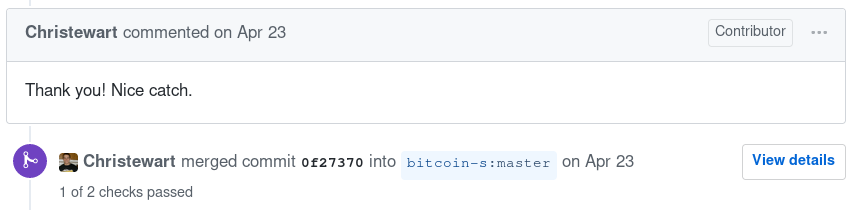
\includegraphics[scale=0.5]{images/bitcoin-s-pr-comment.png}
	\caption{Nice catch comment on our PR \#435 on GitHub}
	\label{fig:output1}
\end{figure}

Here is the relevant code of checkTransaction again:
\begin{lstlisting}[language=scala]
  val prevOutputTxIds = transaction.inputs.map(_.previousOutput.txId)
  val noDuplicateInputs = prevOutputTxIds.distinct.size == prevOutputTxIds.size
\end{lstlisting}

What happens if we have two TransactionOutPoints (previousOutputs) with a different index but referencing the same Transaction ID (txId)?

According to the Bitcoin protocol this is possible.
A transaction can have multiple outputs that should be referenceable by the next transaction.
So this is clearly a bug.

What should not be possible is a transaction referencing the same output twice.
This bug occurred in Bitcoin Core known as CVE-2018–17144 which was patched on September 18, 2018. \cite{cve201817144}

Here, Bitcoin-S did a bit too much and marked all transaction as invalid, if they referenced the same transaction twice.
The fix is, to check on TransactionOutPoint instead of TransactionOutPoint.txId, because TransactionOutPoint contains the txId as well as the output index it references.
So in pseudo code, we check on the tuple (tx, index) instead of (tx).
The fixed code:
\begin{lstlisting}[language=scala]
  val prevOutputs = transaction.inputs.map(_.previousOutput)
  val noDuplicateInputs = prevOutputs.distinct.size == prevOutputs.size
\end{lstlisting}

Since TransactionOutPoint is a case class and Scala has a built in == for case classes there is no need to implement TransactionOutPoint.==.
\begin{figure}[H]
	\centering
		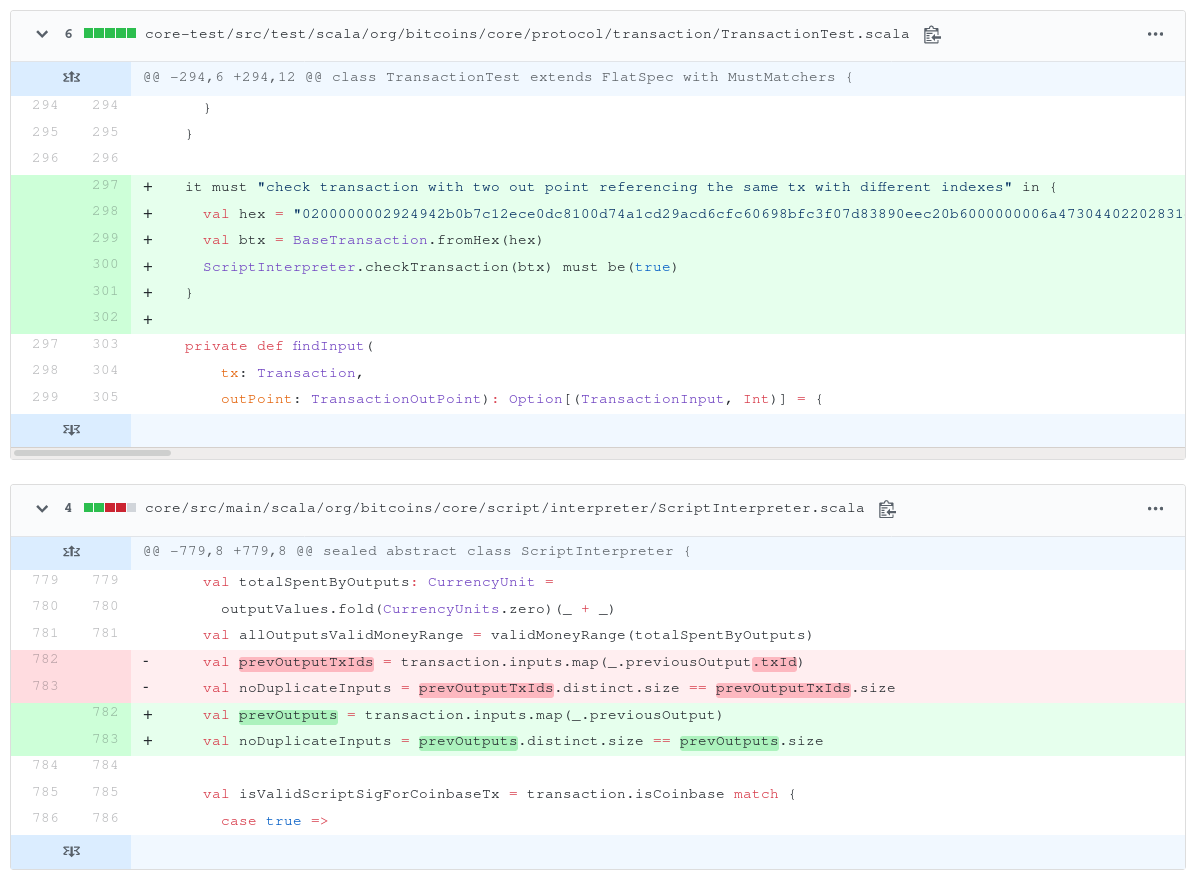
\includegraphics[scale=0.396]{images/bitcoin-s-pr.png}
	\caption{Line changes for PR \#435 from GitHub}
	\label{fig:output1}
\end{figure}

This was fixed in \href{https://github.com/bitcoin-s/bitcoin-s/pull/435}{pull request \mypound435} on GitHub at April 23, 2019, through this work along with a unit test to prevent this bug from appearing again in the future.


\section{Adjusting No-Inflation Property}

\todo{anna: what does it mean to integrate}

Trying to integrate Stainless in Bitcoin-S caused a lot of troubles, mainly because of version conflicts.
For more details see chapter \ref{chap:appendix_arb}.

After integrating Stainless in Bitcoin-S, there were many errors.
It takes too much time to fix them all so it should be easier to extract the classes needed for the \texttt{checkTransaction} function.
\todo{anna: which errors?}

The extracted code has more than 1500 lines.
After running Stainless on it, it still throws a huge bunch of errors about what Stainless can not reason about.
After fixing some of those errors, there appear new ones.
So this would require changing nearly everything of the extracted code.

Let's adjust the property from the \nameref{property_1} to the \nameref{property_2}, because there is not enough time to fix all these errors and write the verification.
This is way less interesting to verify but gives still many insights in what needs to be done to verify some parts of Bitcoin-S and other source code.

So let's look at the \nameref{property_2}.
